\chapter{Category combination strategy}
\label{s:category-combination-strategy}
\is{language strategy!for colour!category combination strategy}
\is{category combination strategy|see{language strategy}}

Some languages also allow users to compound two colour categories into
a new one. This can also be applied to the domain of colour,
especially to describe a colour sample that is not a good example of
any of the basic colour terms.  An example in English would be
\textit{blue-green}. This compounding can also be modulated by an
additional marker, like for example \textit{-ish} in English as in
\textit{brownish-red}. Other languages, such as Vietnamese, allow to repeat
one colour term to give it emphasis, as in \textit{yellow yellow}
\citep{alvarado02modifying}.

\cite{safuanova07russian} have collected data on the focal colours of
compounds in Russian. One of their main findings is that in Russian,
the order in which colour terms are combined has an influence on the
resulting focal colour: the second term seems to be more important in
the expression. This is illustrated in \figref{f:ccs-russian}. The
colours between \textit{\v z\"eltyj} (`yellow') and \textit{zel\"eno} (`green') are
for example named: \textit{zelenovato-\v z\"eltyj} (`greenish-yellow'),
\textit{zel\"eno-\v z\"eltyj} (`green-yellow'), \textit{\v z\"elto-zel\"enyj}
(`yellow-green') and \textit{\v z\"eltovato-zel\"enyj} (`yellowish-green')
where the suffix \textit{-ato} acts as a modulator.

\begin{figure}[htbp]
  \begin{center}
    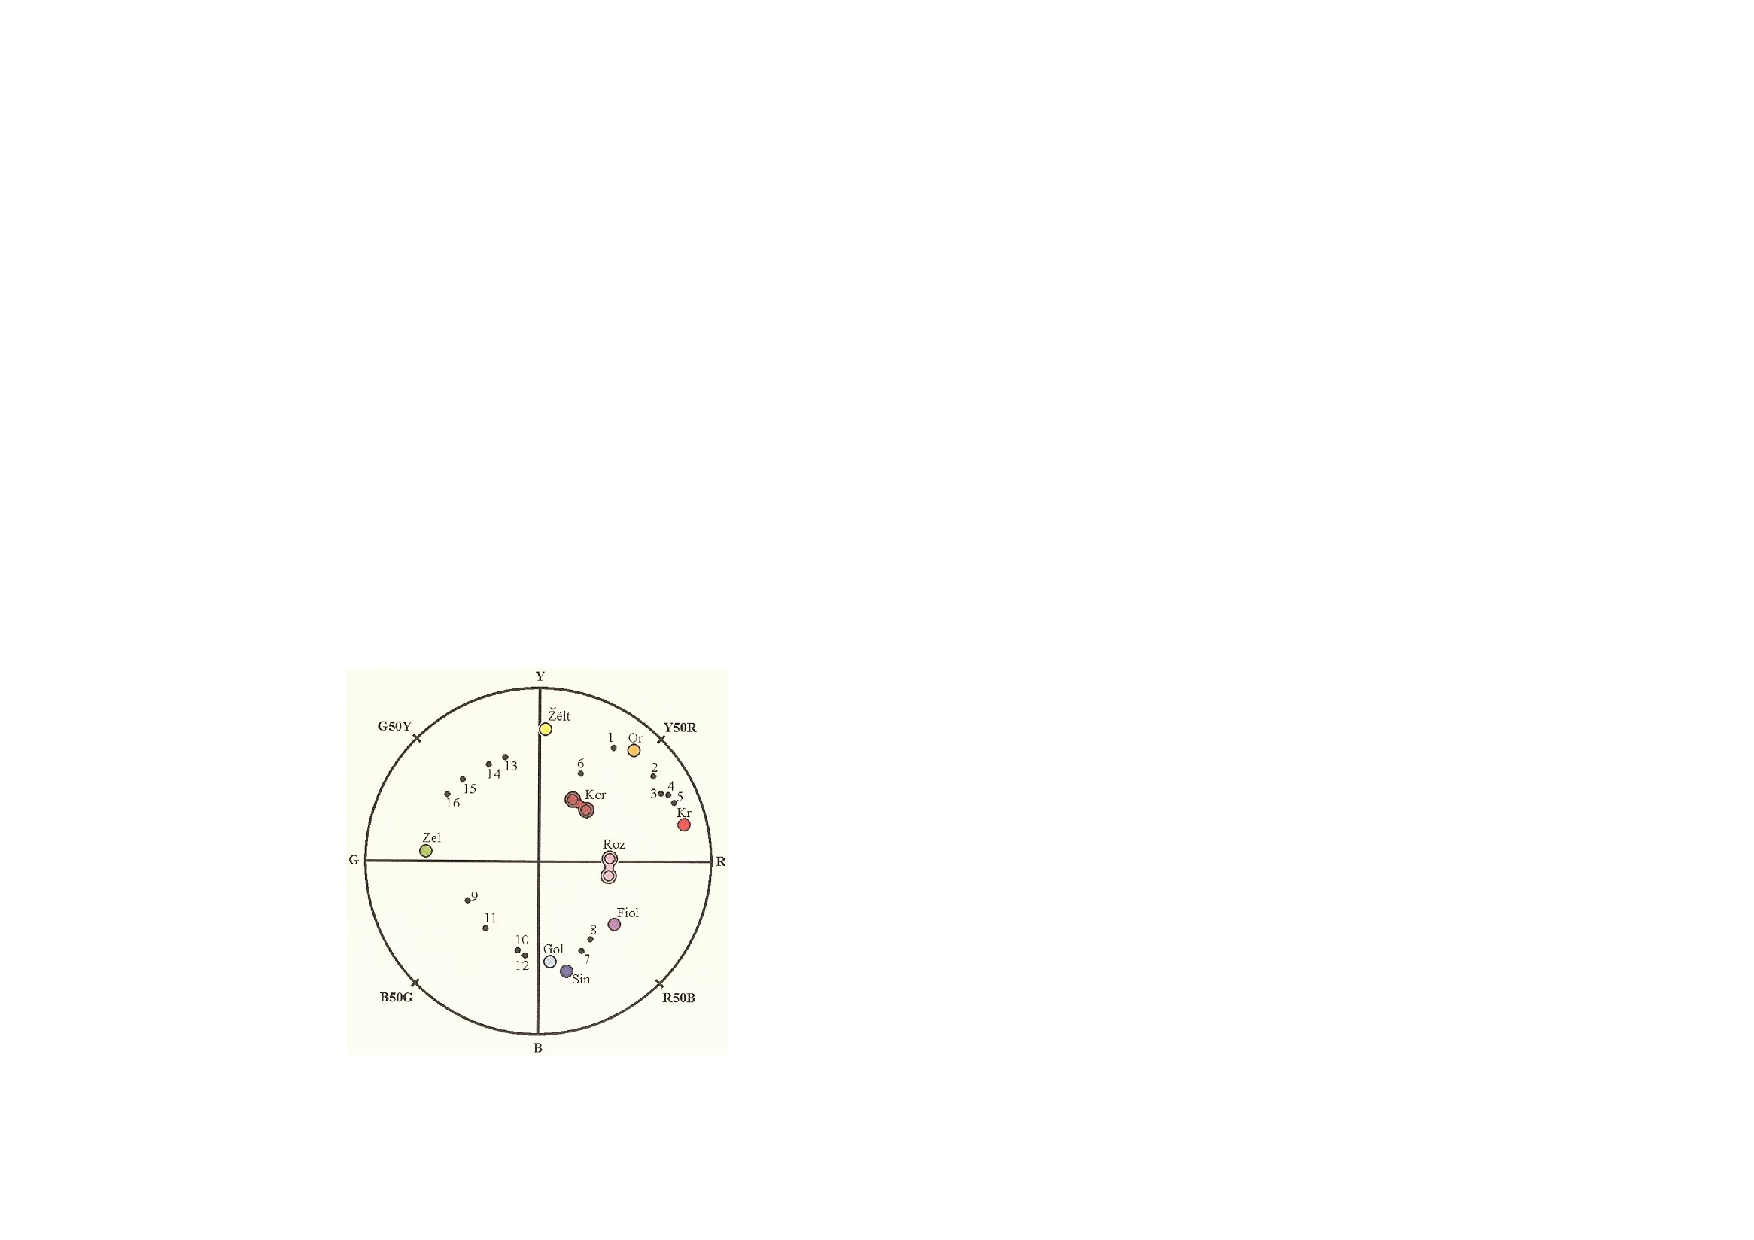
\includegraphics[width=0.6\textwidth]{./category-combination/figures/russian-combination.pdf}
    \caption[Compound chromatic terms in Russian]{Compound chromatic
      terms projected on the hue plane of the NCS colour space. The
      second term in the compound clearly has a bigger impact on the
      resulting focal colour than the first one. The colours between
      \textit{\v z\"eltyj} (`yellow') and \textit{zel\"enyj} (`green') are for
      example named: (13) \textit{zelenovato-\v z\"eltyj}
      (`greenish-yellow'), (14) \textit{zel\"eno-\v z\"eltyj} (`green-yellow'),
      (15) \textit{\v z\"elto-zel\"enyj} (`yellow-green') and (16) \textit{\v z\"eltovato-zel\"enyj} (`yellowish-green'). Figure from
      \cite{safuanova07russian}.}
    \label{f:ccs-russian}
  \end{center}
\end{figure}

To summarise, I have to account for three basic observations: category
combination can be asymmetrical in the sense that one colour category
is deemed more important than the other. This combination can be
modulated through markers in language and the same colour category can
be repeated in the same utterance to give emphasis to indicate it is a
good example of a particular colour category.

\section{Related research}
\label{s:ccs-related-research}

Several suggestions have been made on how the combination of concepts
should be modelled. In certain situations, some compatible properties
can be changed in the base concept, such as in \textit{green apple}. In
other situations, the mapped properties are not compatible and
overrule the corresponding properties in the base concept, such as in
\textit{pink elephant}.

But the combination of concepts is actually not as clear cut, as the
actual modification depends on the context in which it is
used. Consider the Russian example below which states there are many
\textit{red cows} in the Ural mountain range. These cows are of course not
of a bright red colour, but are rather more ginger-coloured
\citep{tribushinina08cognitive}.

\ea
\gll Na Urale mnogo krasnyh korov.\\
On Ural-\textsc{loc} many red-\textsc{pl.gen} cows-\textsc{gen}\\
\glt `There are a lot of red cows in the Urals.'\\
\z


The actual colour implied by the colour adjectives is dependent on
the context in which it is used. The actual colour implied by the
adjective \textit{red} is different whether it is used in the context of
wine, hair, skin, or indeed cows. This is why the use of contrast
classes is suggested. These define a subregion of colours that some
base class is usually associated with, for example the set of all skin
colours. The set of colour categories is transformed into this
subregion. For example, \textit{white skin} does refer to a colour that
would normally be named pinkish and \textit{black} refers to the darkest
colour of skin \citep{gardenfors04conceptual}.

\subsection*{Models}

The colour naming model proposed by
\citeauthor{lammens94computational} sorts all categories based on the
similarity to the colour sample that needs to be named and deployed
some heuristics to include the secondmost similar category using
diminuatives such as \textit{-ish} and \textit{somewhat x-ish}
\citep{lammens94computational}. Other colour naming models store
different centroids for each compound colour term, including the
combination of basic colour terms \citep{mojsilovic05computational}.

\section{Semantic template}
\label{s:ccs-semantic-template}
\is{semantic template!for category combination strategy}

As I am pursuing a compositional approach to semantics, I start from
the semantic network of the basic colour strategy and extend it by
adding a second categorisation process. As the first categorisation
process is strict, it would be unproductive to use the same category
set as it would just return the exact same colour category. In order
for the second categorisation process to be useful, the category set
needs to be modified.

The most naive way to modify the category set is to remove the
category that was used during the first categorisation process. This
would allow the second categorisation process to find the category
that is secondmost similar to the colour sample that needs to be
described. This approach would however not be able to account for 
the repetitive use of the same colour term to highlight the similarity
between the colour sample in the colour category, like in Vietnamese.

The transformation I have implemented is to move all the colour
categories in the colour category set towards the category that has
been used during the first categorisation process. This will entail
that the region of the colour space that was first categorised as the
base category will be repartitioned over its adjacent categories. The
centre of that region, however, will still be classified as the base
category. An illustration of such a transformation is provided in
\figref{f:ccs-semantics-transformation}.

\begin{figure}[htbp]
\centering
\subfigure[]{
  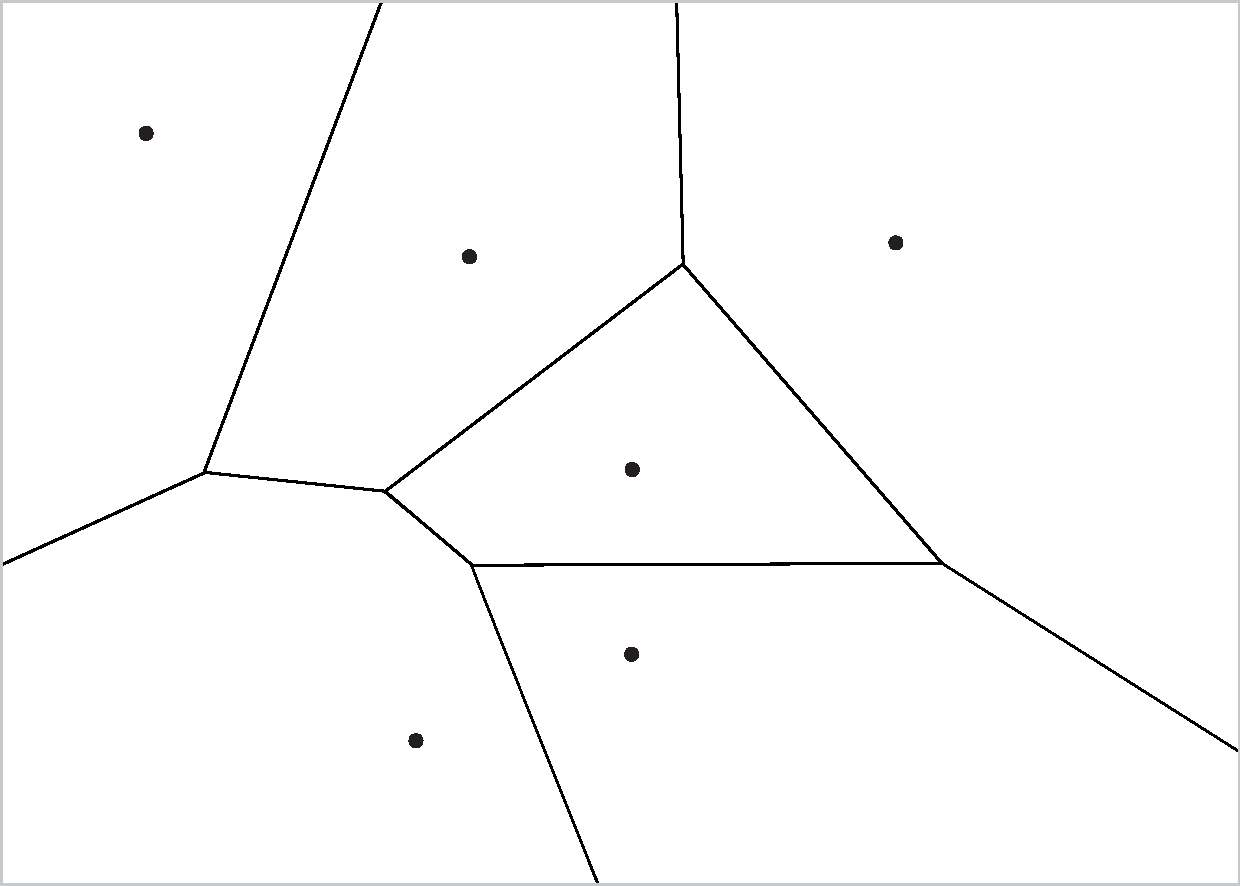
\includegraphics[width=.475\textwidth]{./category-combination/figures/semantics-before-transformation.pdf}
  \label{f:ccs-semantics-before-transformation}
}
\subfigure[]{
  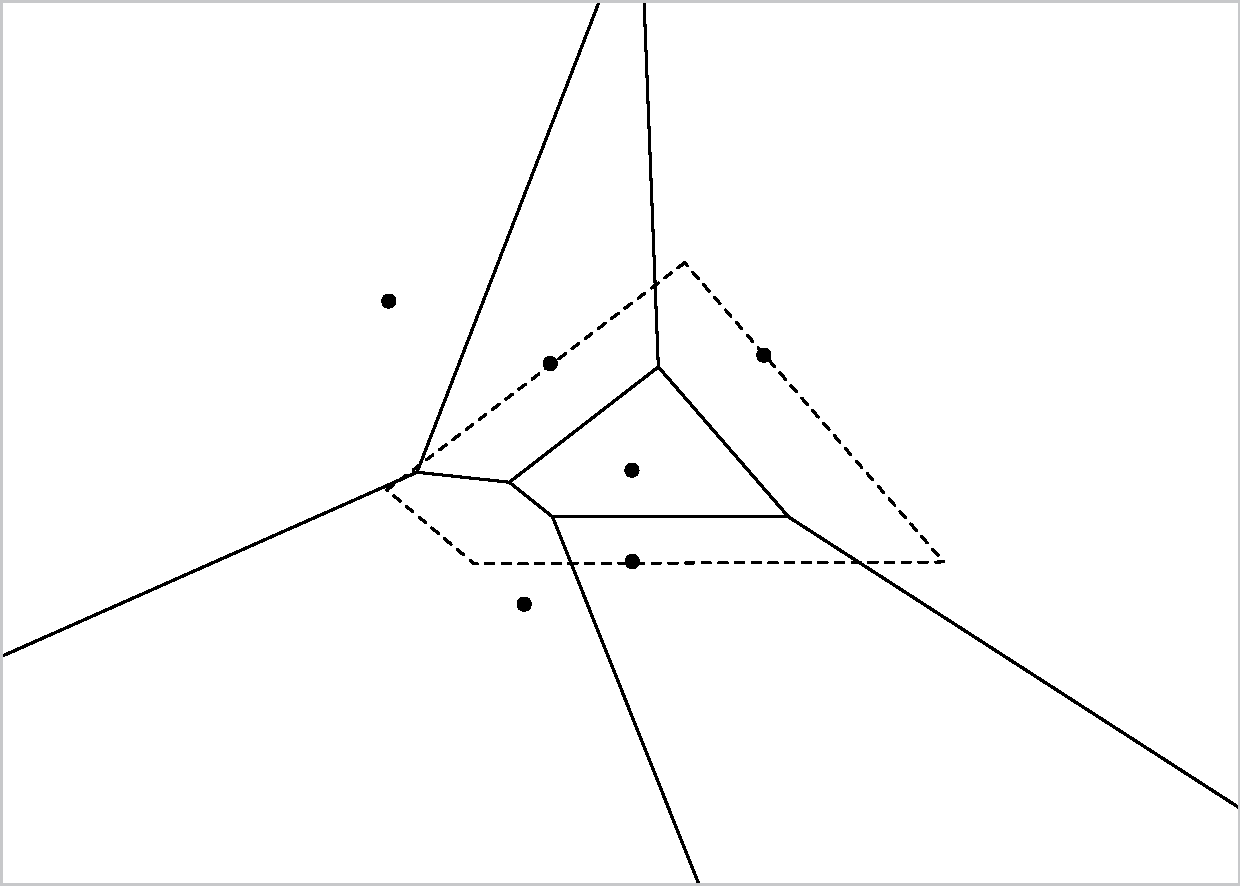
\includegraphics[width=.475\textwidth]{./category-combination/figures/semantics-transformed.pdf}
  \label{f:ccs-semantics-transformed}
}
\caption[Impact of the transformation of the category set in the
category combination strategy on the partitioning of the colour
space]{Impact of the transformation of the category set in the
  category combination strategy on the partitioning of the
  colour space: \subref{f:ccs-semantics-before-transformation}
  partitioning of the colour space before the colour category set is
  transformed; \subref{f:ccs-semantics-transformed} partitioning of
  the colour space after the category set is transformed towards the
  central category. The region that was categorised as
  the base category after the first transformation, is now repartitioned over the categories adjacent
  to the base categories. As the base category is also a member of the
  transformed set, the centre of that region will still be classified
  as the base category.}
\label{f:ccs-semantics-transformation}
\end{figure}

When this second categorisation process would not be constraining
enough to single out a particular colour sample in a context, an
optional categorisation process based on membership can be added.
This process is similar to the one proposed in the graded
  membership strategy but the membership function is now based on the
combined membership of the two categorisation processes instead of
one.

The semantics of the \textsc{category combination strategy} can be
summarised as follows: first all the entities are categorised as in
the basic colour strategy. Next, all categories are drawn
towards the base category that has been used. This transformed
category set is used during the second categorisation
process. Optionally a third categorisation process based on membership
can be added. From the resulting set the entity with the highest
activation is selected.

The proposed semantics satisfy the three requirements outlined at
the beginning of this chapter. Asymmetry is achieved through the
ordering of the categorisation process based on colour: the first one
will define the main region of the conceptual space in which the
sample is to be found; the second one specifies a subregion within
that region. The modulation of the combination process is realised
through the optional categorisation process based on membership. The
repetitive use of a colour category refers to the region that is close
to the repeated colour category.

\subsection{Profiling and first categorisation based on colour}

The profiling and the first categorisation process is identical to the
one of the graded membership strategy. It is a strict
implementation of the categorisation process, as in interpretation
only the samples that are most similar to the interpreted category are
considered for further processing. This decision is based on the
observation that colours that are named using a category combination
will always be most similar to one of its constituent categories, as
supported by the data of Russian compounds \citep{safuanova07russian}.

\subsection{Transformation of the set of colour categories}

The transformation procedure involves moving each colour category
known to the agent in the direction of the base category that was used
during the first categorisation process. Each colour category is moved
to a point on the line segment between the original category and the
base category in the conceptual space of the agent. The new location
is slightly closer to the base category. An illustration of such a
transformation is provided in \figref{f:ccs-semantics-transformation}.

\subsection{Second categorisation based on colour}

The transformed category set is used for a second categorisation based
on colour. In each entity, the resulting membership value of the first
categorisation process is overwritten by the second categorisation
process, but could also be a function based on these two
functions. Although the first categorisation process is important to
select some samples from the context, I have chosen to overwrite the
value as the actual membership of the second categorisation process
is independent of the membership of the first categorisation
process. For example, a \textit{green-blue} colour sample would have a low
membership during the categorisation with the category for blue, but
could be a very good member of the green category that is transformed
for the category for blue.

This process allows for a further specification of the region in the
conceptual space that was originally categorised as the base category.

\subsection{Optional categorisation based on membership}

An optional categorisation process based on membership can be added to
the chain of processes, which would allow for further specification of
the colour sample. As the membership values stored in the entities now
reflect the second categorisation process, this will specify regions
within the regions that were defined by the previous categorised
process.

\subsection{Selection based on activation}

The selection process is based on the notion that each categorisation
process changes the activation values of each of the entities in the
resulting set. The entity with the highest activation is selected as
the entity resulting from the complete process.

\subsection{Semantic constraint network}

The semantic network for the category combination strategy is
shown in \figref{f:ccs-semantic-program}. The
\textsc{Equal-to-Context} and \textsc{Profile-Colour-Dimensions}
primitives are the same as the ones before. The
\textsc{Filter-by-Colour} primitive is like the one introduced before,
but now has a specific argument of the colour category set it is
applying, as this set might be modified by other primitives. This
requires another primitive \textsc{Get-Basic-Colour-Category-Set} to
retrieve all the categories known to the agent to mimic the old
behaviour of \textsc{Filter-by-Colour}. This category set is also
provided to the \textsc{Draw-Category-Set-to-Category} primitive which
draws all the categories in the direction of the category that is used
during the first categorisation process based on colour. Next another
\textsc{Filter-by-Colour} primitive applies the transformed category
set to the sets filtered by its first instantiation. Finally
\textsc{Select-Most-Activated} returns the most activated entity from
this set as the value for the complete process.  An optional
\textsc{Filter-by-Membership} primitive can be added between the last
two primitives (not shown in figure).

\begin{figure}[htbp]
  \centering
  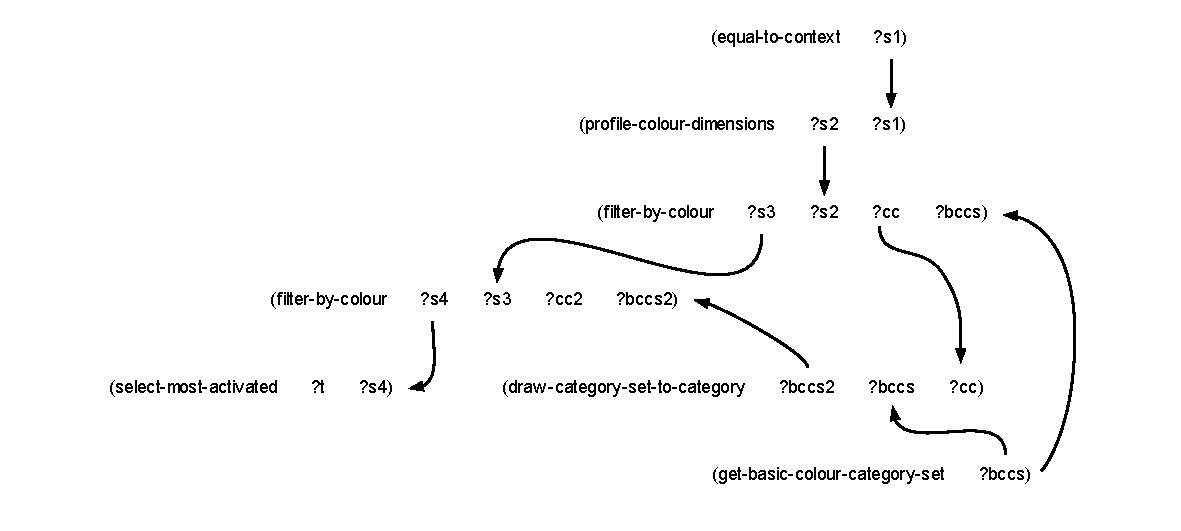
\includegraphics[width=\textwidth]{./category-combination/figures/semantic-program.pdf}
  \caption[The semantic constraint network for the category combination
  strategy]{The semantic constraint network for the category combination
      strategy. Consists of two \textsc{Filter-by-Colour} primitives
    of which the second one deploys a transformed category set. This
    transformation is computed by the
    \textsc{Draw-Category-Set-to-Category} primitive.}
  \label{f:ccs-semantic-program}
\end{figure}

\subsection{Semantic primitives}

\definition{Semantic primitive}{Get-Basic-Colour-Category-Set}

\begin{explanation}{description}
  Retrieves all colour categories known by the agent.
\end{explanation}

\begin{explanation}{slots}
  \verb+?colour-category-set+ (of type category-set)
\end{explanation}

\begin{explanation}{revision specs}
  $\emptyset$: collects all colour categories known to the agent and
  binds it to \verb+?colour-category-set+
\end{explanation}

\definition{Semantic primitive}{Filter-by-Colour}

\begin{explanation}{description}
  Categorises each entity in a source set as the most similar colour
  category in its argument category set. The membership of each entity
  is set to be the similarity to the category it belongs to.
\end{explanation}

\begin{explanation}{slots}
  \verb+?filtered-set+ (of type entity-set) \\
  \verb+?source-set+ (of type entity-set) \\
  \verb+?colour-category+ (of type colour-category) \\
  \verb+?colour-category-set+ (of type category-set)
\end{explanation}

\begin{explanation}{revision specs}
  \verb+?source-set ?colour-category-set+: categorises each entity of
  the source set and returns pairwise bindings for the remaining
  slots; categories to which no entities are assigned, are ignored. \\
  \verb+?source-set ?colour-category-set ?category+: computes the
  categorisation of the source set based on all colour categories in
  the category set and when the resulting set for the provided colour
  category is not empty, it gets bound to \verb+?filtered-set+
\end{explanation}

\definition{Semantic primitive}{Draw-Category-Set-to-Category}

\begin{explanation}{description}
  Draws all categories in a category set towards a particular member
  of this category set. When this category is not a member of this
  set, this operation is undefined.
\end{explanation}

\begin{explanation}{slots}
  \verb+?transformed-category-set+ (of type category-set) \\
  \verb+?category-set+ (of type category-set) \\
  \verb+?category+ (of type colour-category)
\end{explanation}

\begin{explanation}{revision specs}
  \verb+?category ?category-set+: draws all categories in the category
  set towards \verb+?category+ bound to \verb+?category+ so that they
  are on the line segment between of \verb+?category+ and the original
  location of the category; the linear factor that determines the
  resulting position is set to 0.4 (where 0 would be equal to
  \verb+?category+ and 1.0 would be the original location of the
  category)
\end{explanation}

\subsection{Alternative approaches to semantics}

Although not implemented nor tested, it has been suggested that fuzzy
sets could support category combinations in a quite natural way. Some
samples belong with full probability to one fuzzy set representing one
basic colour category, but others will be members of more than one
set. If a sample would have a membership of 0.5 to blue and one of 0.5 to
green, it could be named \textit{blue-green}. The \textit{-ish} suffix could be
used for samples with a high membership of one category and up to a
certain membership of another (e.g. samples with memberships 0.7 to
green and 0.3 to blue could be named \textit{bluish green}
\citep{benavente08parametric}).

\section{Syntactic templates}

The syntactic templates that can be used to express this semantic
network are similar to the templates introduced in the previous
chapter. The main difference to the previous templates is that the
rules don't only need to link the variables of the different entity
sets, but also the variables that deal with colour category sets and
colour categories. This is most clear when observing the arguments of
the \textsc{Draw-Category-Set-to-Category} primitive, which requires
the colour category that is used in the first categorisation process
to compute a new colour category set that will be used during the
second categorisation process. The variables related to colour
categories will be dealt with in the \textsc{colour link},
c-link feature for short.

The linguistic structure for \textit{zel\"eno-\v z\"eltyj} (`green-yellow')
is shown in \figref{f:ccs-linguistic-structure}, in which some
morphological issues are ignored.

\begin{figure}[htbp]
  \centering
  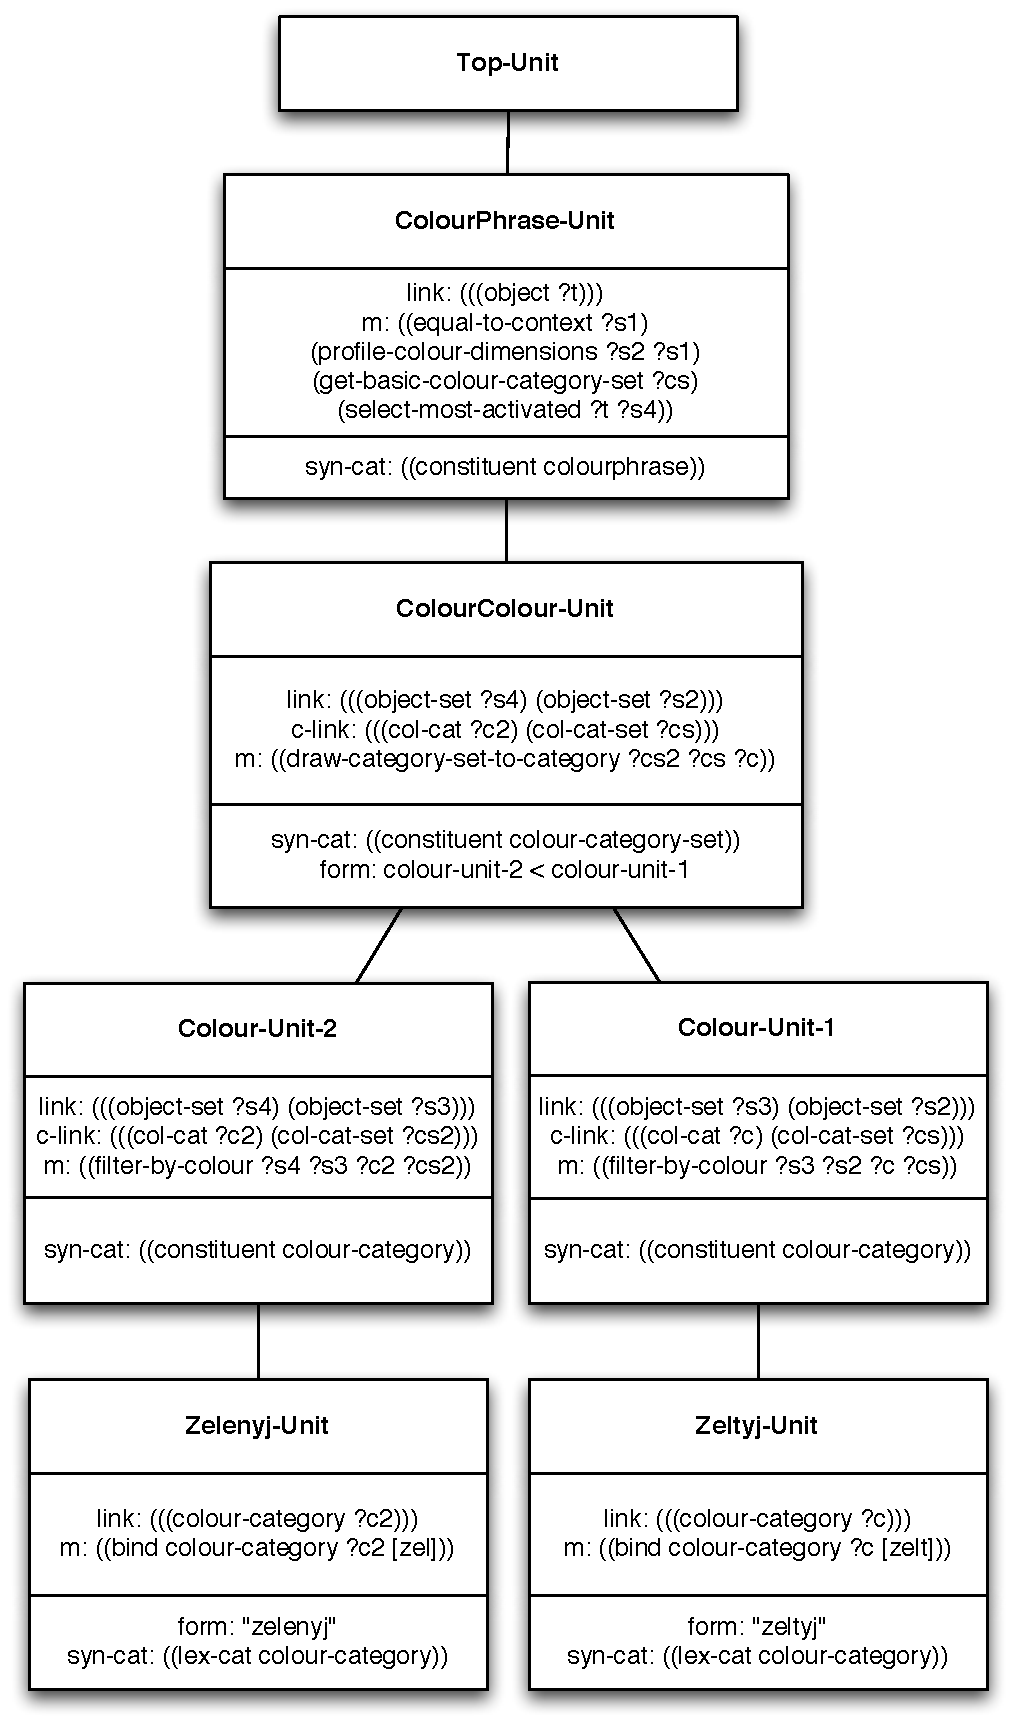
\includegraphics[width=.70\textwidth]{./category-combination/figures/linguistic-structure.pdf}
  \caption[Linguistic structure for category combination
  strategy]{Linguistic structure for category combination
    strategy. Both semantic and syntactic poles are shown in the same
    structure. Semantic information is shown in the top part of each
    unit, the syntactic information in the bottom part of each
    unit. Next to the link features that have been used before to link
    the entity-sets of the primitives together, a c-link feature is
    required to establish variable equalities between primitives for
    the colour categories and the colour category sets.}
  \label{f:ccs-linguistic-structure}
\end{figure}

\subsection{Syntactic template 1.1: Semantic entities}

The semantic entities are dealt with in a similar way as before. I
kindly refer the reader to the previous chapters for examples of
entity rules.

\subsection{Syntactic template 1.2: Functional primitives}
\is{syntactic template!for functional primitives}

The functional rule for \textsc{Filter-by-Colour} is similar to the
one introduced before, but now also provides a c-link feature
in which the variables of its colour category and the colour category
set are stored. The category needs to be available to the rest of the
semantic network for when it should be needed for a transformation of
the colour category set. The colour category set is required to allow
for transformed colour category sets to be used by the filtering
process.

\footnotesize
\ltitle{Functional rule for Filter-by-Colour}
\begin{lstlisting}
((?top-unit
  (sem-subunits (?colour-category-unit)) 
  (tag ?meaning
       (meaning ((filter-by-colour ?s3 ?s2 ?c ?cs)))))
 (?colour-category-unit 
  (link (((colour-category ?c)))))
 ((J ?filter-by-colour-unit ?top-unit (?colour-category-unit))
  ?meaning
  (link (((entity-set ?s3) (entity-set ?s2))))
  (c-link (((colour-category ?c) (colour-category-set ?cs))))))
<-->
((?top-unit 
  (syn-subunits (?colour-category-unit)))
 (?colour-category-unit 
  (syn-cat ((lex-cat colour-category))))
 ((J ?filter-by-colour-unit ?top-unit (?colour-category-unit))
  (syn-cat ((constituent colour-category)))))
\end{lstlisting}
\normalsize

\subsection{Syntactic template 1.3: Contextual primitives}
\is{syntactic template!for contextual primitives}

The basic colour strategy is now redefined 
using the \textsc{Filter-by-Colour} primitive as defined in this
chapter. The contextual rule that is needed for this strategy
is very similar to the contextual rule in \sectref{s:bcs-contextual-primitive}, except that it now also encapsulates
a \textsc{Get-Basic-Colour-Category-Set} primitive of which the argument is part of
the c-link of the subunit.

\footnotesize
\ltitle{ColourPhrase rule for Basic Colour Strategy}
\begin{lstlisting}
((?top-unit
  (sem-subunits (?colour-unit))
  (tag ?meaning
       (meaning ((select-most-activated ?t ?s3)
                 (profile-colour-dimensions ?s2 ?s1)
                 (equal-to-context ?s1)
                 (get-basic-colour-category-set ?cs)))))
 (?colour-unit
  (link (((entity-set ?s3) (entity-set ?s2))))
  (c-link (((colour-category ?c) (colour-category-set ?cs)))))
 ((J ?colourphrase-unit ?top-unit (?colour-unit))
  ?meaning
  (link (((colour-entity ?t))))))
<-->
((?top-unit 
  (syn-subunits (?colour-unit)))
 (?colour-unit 
  (syn-cat ((constituent colour-category))))
 ((J ?colourphrase-unit ?top-unit (?colour-unit))
  (syn-cat ((constituent colourphrase)))))
\end{lstlisting}
\normalsize

\subsection{Syntactic template 2.2: Re-use of constructions}
\is{syntactic template!re-use of constructions}

An extended version of syntactic template 2.1 needs to be
introduced. The resulting rule looks similar to the one introduced
before, but additionally the rule needs to take care of two
additional aspects. First it needs to be able to cover some
meaning. For the current semantic template, this would be the
\textsc{Draw-Category-Set-to-Category} primitive. And second, it needs
to provide the correct colour link of the new unit.

\footnotesize
\ltitle{ColourColour rule}
\begin{lstlisting}
((?top-unit
  (sem-subunits (?unit-2 ?unit))
  (tag ?meaning
       (meaning ((draw-category-set-to-category ?cs2 ?cs ?cc)))))
 (?unit-2
  (link (((entity-set ?s3) (entity-set ?s2))))
  (c-link (((colour-category ?cc2) (colour-category-set ?cs2)))))
 (?unit
  (link (((entity-set ?s2) (entity-set ?s1))))
  (c-link (((colour-category ?cc) (colour-category-set ?cs)))))
 ((J ?colourcolour-unit ?top-unit (?unit-2 ?unit))
  ?meaning
  (link (((entity-set ?s3) (entity-set ?s1))))
  (c-link (((colour-category ?cc2) (colour-category-set ?cs))))))
<-->
((?top-unit
  (syn-subunits (?unit-2 ?unit))
  (tag ?form 
       (form ((meets ?unit-2 ?unit)))))
 (?unit-2 
  (syn-cat ((constituent colour-category))))
 (?unit 
  (syn-cat ((constituent colour-category))))
 ((J ?colourcolour-unit ?top-unit (?unit-2 ?unit))
  ?form
  (syn-cat ((constituent colour-category)))))
\end{lstlisting}
\normalsize

\section{Baseline experiment}
\is{baseline experiment!for category combination strategy}

In the baseline experiment, I will compare three different language
systems. All language systems are based on the Russian basic colour
categories \citep{safuanova07russian}. The first one is based on the
strict version of the basic colour strategy, the second one is
based on the variant of the category combination strategy
without the additional categorisation based on membership and the
third language system is based on the graded variant of this strategy.

The exact location of the chromatic colour terms in Russian have been
determined \citep{safuanova07russian}. These categories were reported
in the Natural Color System and have been converted to the CIE
$L^*a^*b^*$ colour space using the method described in Appendix
\ref{s:NCS}. Only the location of the chromatic colour categories has
been determined which include two hues for the region English speakers
would call \textit{blue}: \textit{sinij} (`dark blue') and \textit{goluboj} (`light
blue'). The basic colour categories are shown in \figref{f:ccs-russian-basic}.

\begin{figure}[htpb]
  \centering
  
\includegraphics[height=1.25cm]{./category-combination/figures/russian-basic-categories.pdf}
  \caption[The basic chromatic colour categories for Russian]{The
    basic chromatic colour categories for Russian based on the work of
    \citeauthor{safuanova07russian}. From left to right: \textit{krasnij}
    `red', \textit{oran\v zevyj} `orange', \textit{\v z\"eltij} `yellow', \textit{zel\"enyj}
    `green', \textit{sinij} `dark blue', \textit{goluboj} `light blue',
    \textit{rozovyj} `rose', \textit{fioletovyj} `purple' and \textit{kori\v cnevyj}
    `brown'.}
  \label{f:ccs-russian-basic}
\end{figure}

The same study reports on the exact location of some chromatic
compounds. As a first qualitative test, I will verify whether the
proposed semantics and syntax will name the reported locations in a
similar way. An example from the study lists the chromatic compounds
between \textit{\v z\"eltyj} (`yellow') and \textit{zel\"enyj} (`green') which are
reproduced in \figref{f:ccs-russian-compounds}.

\begin{figure}[htpb]
  \centering
  
\includegraphics[height=1.25cm]{./category-combination/figures/russian-compounds.pdf}
  \caption[Example of colour compounds in Russian]{Example of colour
    compounds in Russian \citep{safuanova07russian}. From left to
    right: (a) \textit{\v z\"eltyj} `yellow', (b) \textit{zelenovato-\v z\"eltyj} 
    `greenish-yellow', (c) \textit{zel\"eno-\v z\"eltyj} `green-yellow',
    (d) \textit{\v z\"elto-zel\"enyj} `yellow-green', (e) \textit{\v z\"eltovato-zel\"enyj}
    `yellowish-green', (f) \textit{zel\"enyj} `green'.}
  \label{f:ccs-russian-compounds}
\end{figure}

For this naming benchmark, \is{naming benchmark!for category combination strategy}
I use an agent that is knowledgeable about
the basic colour strategy and the category combination
  strategy (both the graded and the ungraded variant) and an implementation of the
basic colour categories of Russian (as shown in \figref{f:ccs-russian-basic}). Next, I run the production procedure and
check what utterances are produced for the chips shown in \figref{f:ccs-russian-compounds}. When more than one strategy is capable
of reaching the communicative goal, the strategy in which the topic
entity has the highest activation is selected. This activation
reflects the membership of the last categorisation process.

The results of this naming benchmark are shown in \tabref{t:ccs-russian-naming-benchmark}. Five out of six colour samples
are named correctly. The one chip that (d) cannot be named is the
yellow-green one. This is due to the first categorisation process
based on colour, which categorises the (a-d) as \textit{\v z\"eltyj}. Only (a-c)
are discriminable by one of the provided language strategies. This
example does not include the morphological complexities of the Russian
language.

\begin{table}[htpb]
  \centering
  \begin{tabular}{l>{\itshape}l>{\itshape}l}
  \lsptoprule
    & \normalfont expected name & \normalfont produced name \\
    \midrule
    (a) & \v z\"eltyj & zeltyj \\
    (b) & zelenovato-\v z\"eltyj  & zelenyj -ato zeltyj \\
    (c) & zel\"eno-\v z\"eltyj & zelenyj zeltyj \\
    (d) & zelto-zelenyj & \normalfont -- \\
    (e) & \v z\"eltovato-zel\"enyj & zeltyj -ato zelenyj \\
    (f) & zel\"enyj & zelenyj \\
    \lspbottomrule
  \end{tabular}
  \caption[Naming benchmark for Russian colour compounds]{Naming benchmark for Russian colour compounds. Five out of six samples are named correctly. The one sample that can not be named is wrongly categorised as \textit{zeltyj} during the first categorisation process based on colour.}
  \label{t:ccs-russian-naming-benchmark}
\end{table}

\begin{figure}[p]
  \centering
  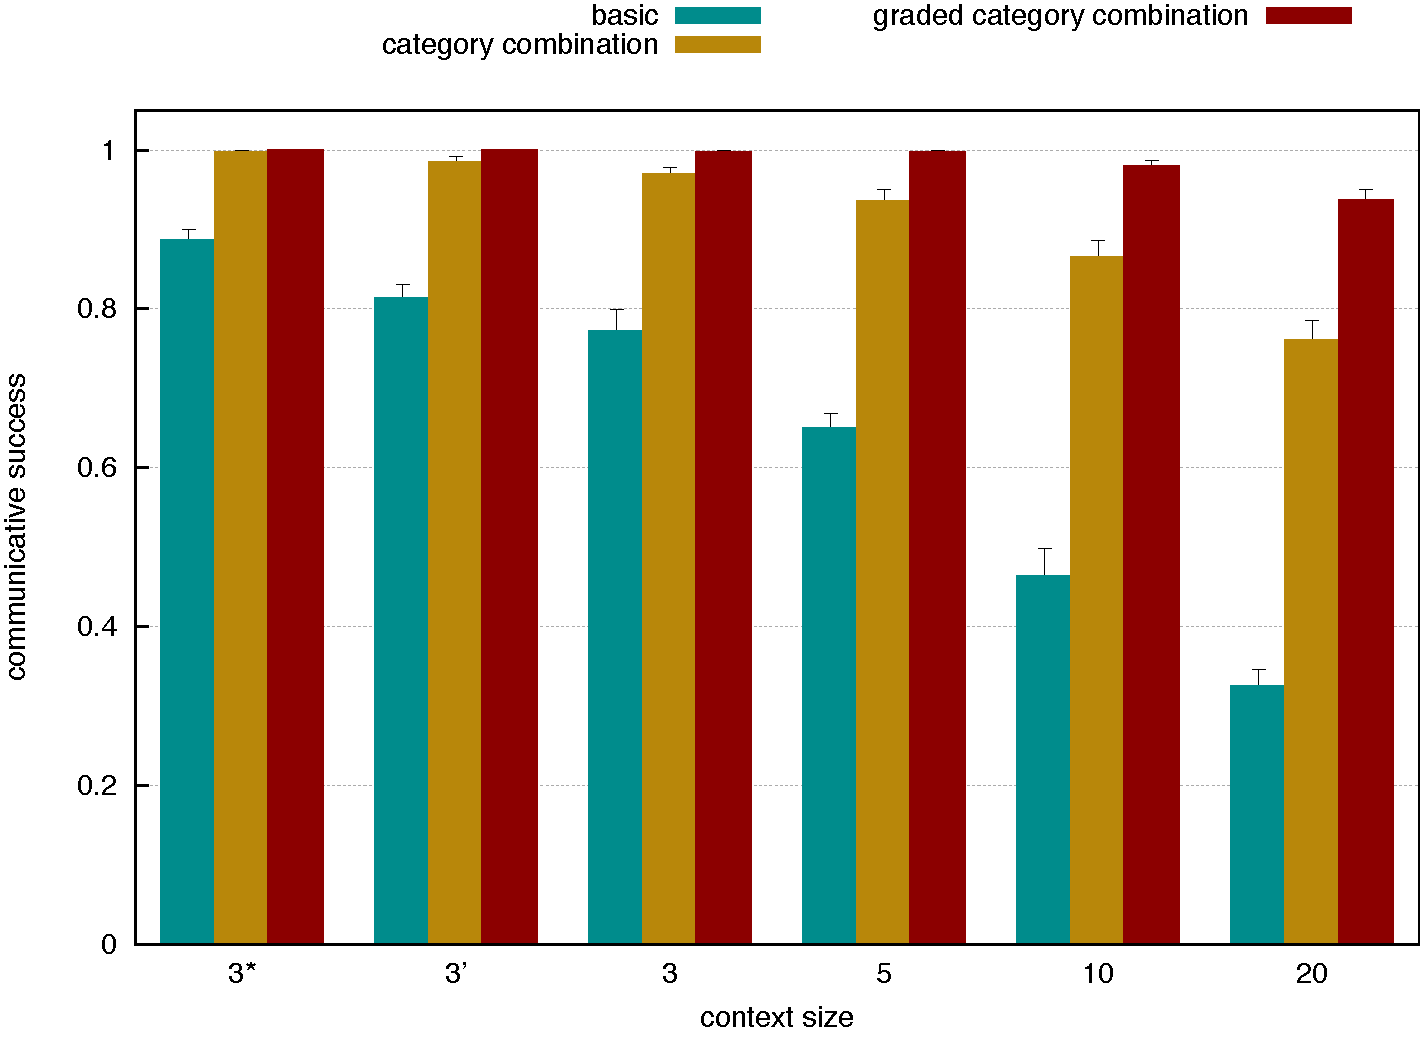
\includegraphics[width=.8\textwidth]{./category-combination/figures/baseline.pdf}
  \caption[The baseline communicative success for category combination
  strategy]{The baseline communicative success for category
    combination strategy, comparing three different language systems
    based on Russian (9 terms). The first system is based on the basic
    colour strategy, the second on the category combination strategy
    and the third one on the graded category combination
    strategy. Allowing agents to combine basic categories results in
    higher communicative success. This effect is increased by adding
    another categorisation process based on membership.}
  \label{f:ccs-baseline}
\end{figure}

\subsection*{Results}

The resulting baseline communicative success is shown in \figref{f:ccs-baseline}. The communicative success for the system in
which agents are allowed to combine categories is higher than when
they are restricted to their basic usage. The communicative success
for the system in which an additional categorisation process based on
the membership is added, is even higher. The richer the semantics the
agents are allowed to use, the higher the resulting communicative
success.

As the number of colour samples in one context increases, the
performance of each of the strategies decreases. The basic
  colour strategy is most prone to this phenomenon. Being able to
combine colour categories compensates for most of the loss. An
additional categorisation process based on membership results in a
language system that is quite successful, even in very large contexts.

Compared to the English basic colour system (shown in \figref{f:gms-baseline}), the baseline communicative success for Russian
is lower. This is due to the lower number of basic colour categories
that are reported for the Russian system (9 compared to 11 for
English). The study on Russian colour categories only reports on
chromatic colour categories, and therefore does not specify locations
of the achromatic colour categories (white, grey and black).


\section{Conclusion}

In this chapter, I have introduced a compositional semantics for the
category combination strategy and linguistic rules to express
this semantics in language. Using a naming benchmark, I have
qualitatively compared the resulting names to these reported for the
Russian language. I have shown the positive impact of combining
colour categories on the baseline communicative success. This impact
was even higher when the category combination process was extended
to include a categorisation process based on membership.

\newpage
\thispagestyle{empty}
